


Progression sivuun uusien mitattavien arvojen lisääminen on rikkonut raportin teko ominaisuuden.
Tämän hetkinen raportin teko hakisi käyttäjän mitattavan suureen ja sen alku ja lopputuloksen.
Raportin teossa pitäisi pystyä valita mitä mitattavia arvoja halutaan raporttiin.
\medskip


Raportti pitää tehdä yhteensopivaksi useamman mitattavan arvon kanssa.
Raportti dokumentin rakennus koodia pitää muokata siten että se tukisi useampaa mitattavaa arvoa.
Raportinteko käyttöliittymää pitää muokata siten, että siitä voi päättää mitä mitattavia arvoja halutaan raporttiin.


\subsection*{Raportti dokumentin luonti}

% selitä export vähän paremmin
Raportti dokumentti on toteutettu CSV tietomuotoon. 
CSV tiedostoja on helppo rakentaa ja niihin on helppo lisätä rivejä ja sarakkeita.
Koska mitattavien arvojen suureet ovat merkkijono listassa voimme käyttää forEach funktiota ja konkatenoida käyttäjän mitattavat arvot merkkijonona dokumenttiin.
\medskip


Raportti ominaisuus on saatavilla vain käyttäjille joilla on siihen käyttöoikeudet.
Käyttäjän roolit varmistetaan selaimella ja palvelimella.
Käyttäjä ei pääse raportinteko sivulle ellei hänellä ole oikeitä käyttöoikeuksia,
ja kun käyttäjä hakee raporttiin käytettyä dataa, palvelin metodi varmistaa käyttäjän roolit.
CSV rakennetaan itse selaimella, joten suurien dokumenttien rakentaminen ei hidastaisi palvelinta.




\subsection*{Käyttöliittymä}


Raportin teko käyttöliittymään pitää lisätä tapa jollla käyttäjä voi valita mitä mitattavia suurteita hän haluaa raporttiin.
Lisäsin käyttöliittymään listan johon käyttäjä voi lisätä tekstikenttiä.
Näihin tekstikenttiin voidaan antaa mitattavan arvon suure merkkijonona. 
Tämä lista annetaan palvelimen raportinteko metodille argumenttina, joten metodi voi hakea käyttäjien tarvittavat mitattavat arvot.
Lista on toteutettu tilallisena komponenttina.



\bigskip
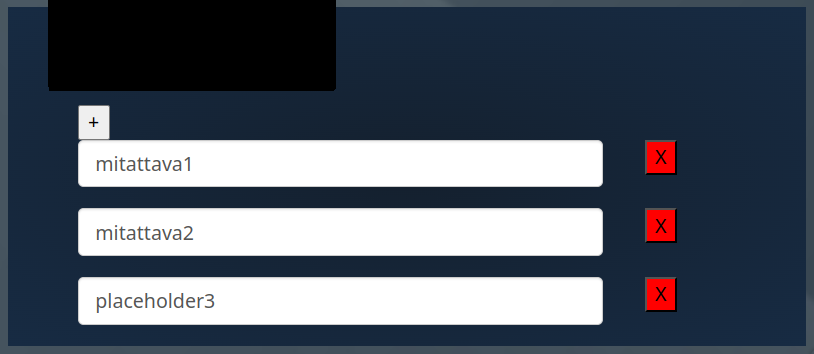
\includegraphics[width=15cm]{src/public/measutableEdited.png}\\
kuva käyttöliittymään liisätystä komponentista
\medskip




\subsection*{Yhteenveto}

Käyttöliittymmään lisätyyn komponenttiin voidaan lisätä niin monta mitattavaa arvoa kun käyttäjä haluaa.
Kenttiä voidaan myös poistaa punaisesta X napista.
Kun päivitin käyttäjän luomis valikkoa progressio ominaisuudelle tein komponentin, josta voi lisätä mitattavia arvoja käyttäjälle.
Uudelleen käytin tätä komponenttia raportinteko sivulla.
Tämä nopeutti työtä huomattavasti ja tuo esille React komponenttien uudelleen käytettävyyden.
Olin alkuperin tehnyt komponentista uudelleenkäytettävän jos sen tarve olisi tullut, 
joten huolellinen suunnittelu aijemmin säästi aikaa tulevaisuudessa.

\medskip

Työ raportin teko ominaisuuden korjaamiseen ei ollut suuri,
mutta tämä kokemus kertoo miten muutokset ominaisuuksiin voivat vaikuttaa muihin alueisiin koodipohjassa.
Tämä pitää ottaa huomioon kun toteuttaa ominaisuuksia,
ominaisuus pitäisi olla helposti ymmärrettävissä, 
joten muutokset muihin ominaisuuksiin vaatisi mahdollisimman vähän korjauksia koodipohjan muihin osaalueisiin.




